%%%%%%%%%%%%%%%%%%%
%%% 2023-08-17 %%%%
%%%%%%%%%%%%%%%%%%%
\section{Introducción y generalidades (2023-08-17)}
\begin{frame}\frametitle{Contexto y definiciones}
  \begin{itemize}
  \item La palabra \textit{robot} tiene su origen en la obra \textit{Rossum's Universal Robots} del escritor checo $Karel \,\check{C}apeck$, publicada en 1921, y su significado es ``trabajo duro''.
  \item Latombe (1991) define un robot como un dispositivo mecánico versátil equipado con sensores y actuadores bajo el control de un sistema de cómputo \cite{Latombe1991MotionPlanning}.
  \item Arkin (1998) propone que un robot inteligente es una máquina capaz de extraer información de su ambiente y usar el conocimiento acerca de su mundo para moverse de manera segura y significativa, con un propósito específico \cite{Arkin1998BehBasedRobo}.
  \item Robótica es la ciencia que estudia la conexión inteligente entre la percepción y la acción. 
  \end{itemize}
\end{frame}

\begin{frame}\frametitle{Áreas de la Robótica}
  
  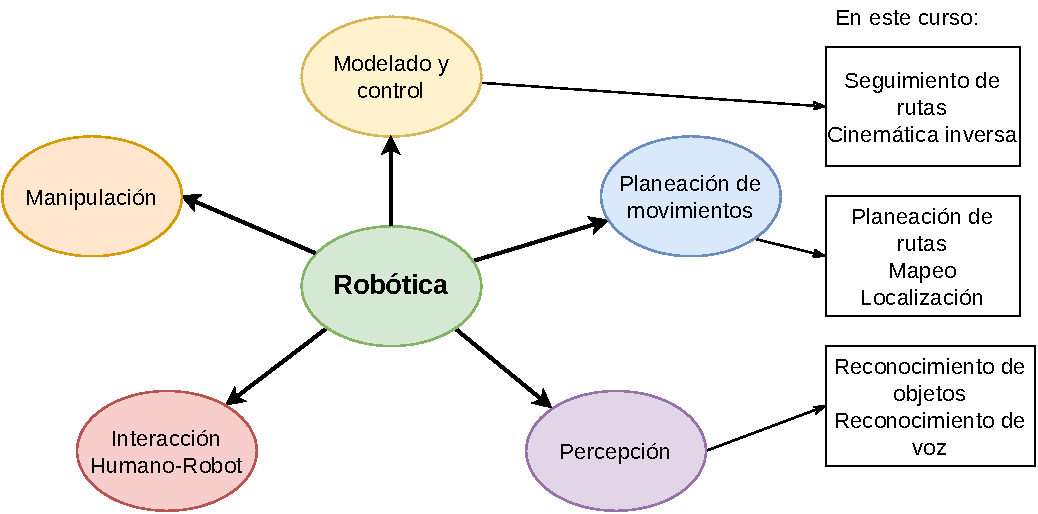
\includegraphics[width=0.9\textwidth]{Figures/RoboticsAreas.pdf}
\end{frame}

\begin{frame}\frametitle{Componentes de un robot}
  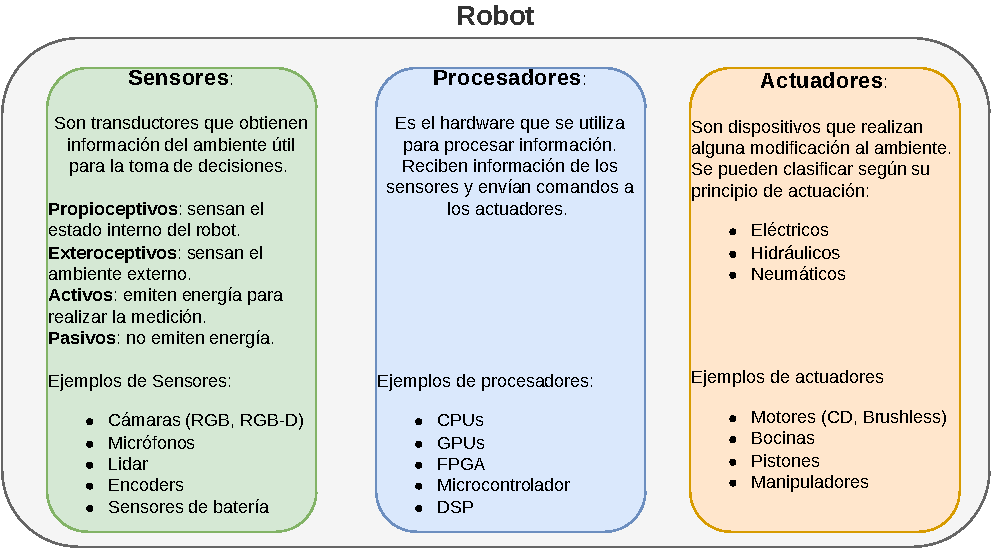
\includegraphics[width=0.9\textwidth]{Figures/RobotComponents.pdf}
\end{frame}

\begin{frame}\frametitle{Conceptos Básicos}
  \begin{itemize}
  \item \textbf{Configuración:} es la descripción de la posición en el espacio de todos los puntos del robot. Se denota con $q$.
  \item \textbf{Espacio de configuraciones:} es el conjunto $Q$ de todas las posibles configuraciones. 
  \item \textbf{Grados de libertad:} número mínimo de variables independientes para describir una configuración. En este curso, la base móvil del robot tiene 3 GdL, la cabeza tiene 2 GDL y cada brazo tiene 7 GDL más 1 GdL para el gripper. En total, el robot tiene 21 GdL. 
  \end{itemize}
  \textbf{Propiedades del robot:}
  \begin{itemize}
  \item \textbf{Holonómico:} el robot puede moverse instantáneamente en cualquier dirección del espacion de configuraciones. Comunmente se logra mediante ruedas de tipo \textit{Mecanum} u \textit{Omnidireccionales}. 
  \item \textbf{No holonómico:} existen restricciones de movimiento en velocidad pero no en posición. Son restricciones que solo se pueden expresar en términos de la velocidad pero no pueden integrarse para obtener una restricción en términos de posición. Ejemplo: un coche sólo puede moverse en la dirección que apuntan las llantas delanteras, sin embargo, a través de maniobras puede alcanzar cualquier posición y orientación. El robot de este curso es no holonómico. 
  \end{itemize}
\end{frame}

\begin{frame}\frametitle{Conceptos Básicos}
  \textbf{Propiedades de los algoritmos:}
  \begin{itemize}
  \item \textbf{Complejidad:} cuánta memoria y cuánto tiempo se requiere para ejecutar un algoritmo, en función del número de datos de entrada (número de grados libertad, número de lecturas de un sensor, entre otros).
  \item \textbf{Optimalidad:} un algoritmo es óptimo cuándo encuentra una solución que minimiza una función de costo.
  \item \textbf{Completitud:} un algoritmo es completo cuando garantiza encontrar la solución siempre que ésta exista. Si la solución no exite, indica falla en tiempo finito.
    \begin{itemize}
    \item Completitud de resolución: la solución existe cuando se tiene una discretización. 
    \item Completitud probabilística: la probabilidad de encontrar la solución tiende a 1.0 cuando el tiempo tiende a infinito.
    \end{itemize}
  \end{itemize}
  Una explicación más detallada se puede encontrar en el Cap. 3 de \cite{choset2005principles}.
\end{frame}

\begin{frame}\frametitle{Primitivas de la robótica}
Las tareas que puede llevar a cabo un robot se pueden clasificar en tres grandes conjuntos conocidos como primitivas de la robótica: sensar, planear y actuar.
  \begin{itemize}
  \item \textbf{Sensar: } extracción de información del ambiente interno o externo del robot.
  \item \textbf{Planear: } generación de subtareas y toma decisiones a partir de la información de los sensores y/o de alguna Representación intenra del ambiente.
  \item \textbf{Actuar: } modificación del ambiente con alguno de los dispositivos del robot. 
  \end{itemize}
\end{frame}

\begin{frame}\frametitle{Paradigmas de la robótica}
  \textbf{Paradigma jerárquico.} Las tres primitivas se realizan en forma secuencial.
  \begin{figure}
    \centering
    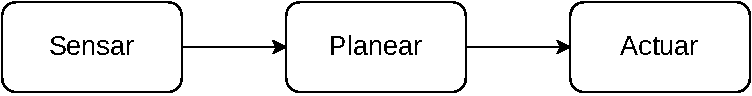
\includegraphics[width=0.7\textwidth]{Figures/ParadigmHierarchical.pdf}
  \end{figure}
  \begin{itemize}
  \item Fuerte dependencia de una representación interna del ambiente
  \item Tiempo de respuesta lento comparado con el paradigma reactivo
  \item Alto costo computacional
  \item Se pueden resolver tareas con alto nivel cognitivo
  \item Alta capacidad de predicción
  \end{itemize}
\end{frame}

\begin{frame}\frametitle{Paradigmas de la robótica}
  \textbf{Paradigma reactivo.} El sensado y la actuación se conectan directamente sin que haya de por medio una planeación.
  \begin{figure}
    \centering
    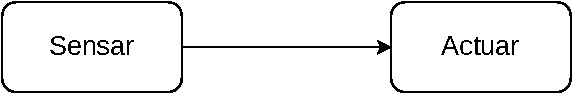
\includegraphics[width=0.5\textwidth]{Figures/ParadigmReactive.pdf}
  \end{figure}
  \begin{itemize}
  \item No requiere una representación interna del ambiente
  \item Tiempo de respuesta rápido comparado con el paradigma jerárquico
  \item Bajo costo computacional
  \item En general, no se pueden resolver tareas con alto nivel cognitivo
  \item Baja capacidad de predicción
  \end{itemize}
\end{frame}

\begin{frame}\frametitle{Paradigmas de la robótica}
  \textbf{Paradigma híbrido.} Tiene como objetivo utilizar las ventajas de ambos paradigmas, es decir, emplear comportamientos reactivos para que el robot responda rápidamente ante cambios en el ambiente sin perder la alta capacidad cognitiva y de predicción que brinda el paradigma jerárquico
  \begin{figure}
    \centering
    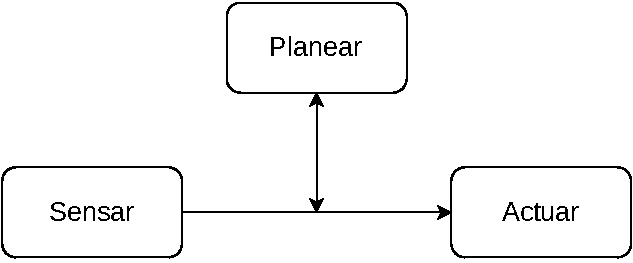
\includegraphics[width=0.5\textwidth]{Figures/ParadigmHybrid.pdf}
  \end{figure}
\end{frame}

\begin{frame}[containsverbatim]\frametitle{Tarea 1 - Herramientas de software}
  \begin{enumerate}
  \item Abrir cuenta en GitHub (si no se tiene) y enviar el nombre de usuario por correo electrónico. 
  \item Instalar y correr el software del curso de acuerdo con las instrucciones del repositorio\\ \url{https://github.com/mnegretev/Mobile-Robots-2024-1} (se puede hacer una instalación nativa o usar la máquina virtual).
  \item Abrir el archivo \texttt{Mobile-Robots-2024-1/catkin\_ws/src/hri/justina\_gui/src/MainWindow.ui} y modificar la línea 14 para que diga:
    \begin{lstlisting}[language=html,firstnumber=14]
      <string>Mobile Robots - NOMBRE COMPLETO</string>
    \end{lstlisting}
  \item Recompilar y ejecutar de acuerdo con las instrucciones del repositorio.
  \end{enumerate}
  \textbf{Entregables:}
  \begin{itemize}
  \item Código modificado en la rama correspondiente
  \item Capturas de pantalla del visualizador RViz y del Simulador Gazebo corriendo el software del curso
  \item Captura de pantalla de la GUI con la modificación del punto anterior. 
  \end{itemize}
  \textbf{Deadline: } 2023-08-24 al inicio de la clase. 
\end{frame}
